\section{Grundlagen}
Wir beginnen mit einem Überblick über das Problem und die Zielgruppe unserer Kunden.
Anschliessend führen wir grundlegende Begriffe ein, die für das Verständnis unseres Projekts
wichtig sind. Im nächsten Schritt betrachten wir ähnliche Projekte, die vergleichbare Herausforderungen adressieren.
Da wir Fiducial Marker zur Erkennung der Anschlagpunkte verwenden, erläutern wir die Grundlagen zur 
Erkennung dieser Marker sowie zur Bestimmung ihrer Position relativ zur Kamera. Wir werden ausserdem eine Einführung in 
Kamera-Hardware geben und erläutern, warum deren Kalibrierung vor den Berechnungen von entscheidender Bedeutung ist.
Abschliessend stellen wir die Frameworks vor, die im Projekt verwendet wurden.

\subsection{Problemstellung}
Ludwig System, ein Hersteller von Werkzeugen für Baustellen, entwickelt derzeit eine autonome Traverse. Damit diese 
Traverse autonom agieren kann, müssen drei wesentliche Ziele erreicht werden: die automatische Erkennung einer Last, 
die mechanische Ausrichtung der Traverse basierend auf der erkannten Last und den Anschlagspunkten sowie die Verriegelung 
der Haken an den Anschlägen. Während Ludwig System die Entwicklung der letzten beiden Schritte übernimmt, konzentriert sich
unsere Arbeit auf die Erfüllung des ersten Schrittes. Hierbei geht es um die Auswahl geeigneter Sensoren und die Implementierung
praktikabler Methoden, die es der Traverse ermöglichen, Lasten und Anschlagspunkte zu erkennen. Zur besseren Verständlichkeit der 
folgenden Ausführungen werden im nächsten Schritt die relevanten Schlüsselbegriffe definiert.


\subsubsection{Anwendungsdomäne}
Das Abhängen von Lasten per Hand ist nicht nur zeitaufwendig, sondern oft auch gefährlich. 
Ludwig System bietet mit ihren funkgesteuerten Lasthaken eine innovative Lösung, 
die diese Arbeit deutlich erleichtert. Diese Haken ermöglichen es den Mitarbeitenden, 
Lasten aus sicherer Entfernung anzuheben und auszubalancieren. Besonders beliebt ist 
die Traverse, die speziell für den Transport von Dachelementen und Wänden entwickelt wurde. 
Allerdings müssen aktuelle Versionen noch manuell an die Last befestigt werden, 
was besonders bei hohen Wänden zeitaufwendig und gefährlich sein kann. 
Abbildung \ref{fig:ludwig} illustriert die Nutzung der Traverse und des Haken.

\begin{figure}[H]
    \centering
    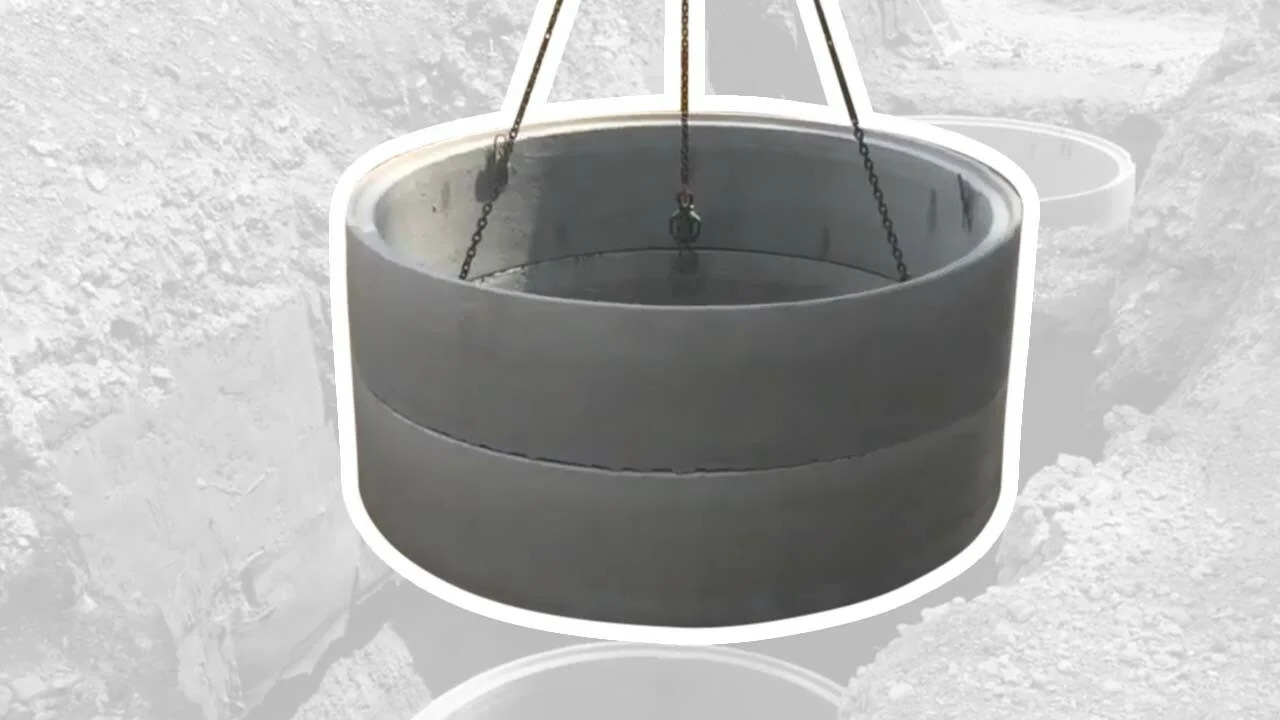
\includegraphics[width=0.5\textwidth]{graphics/Betonelement.jpg}\hfill%
    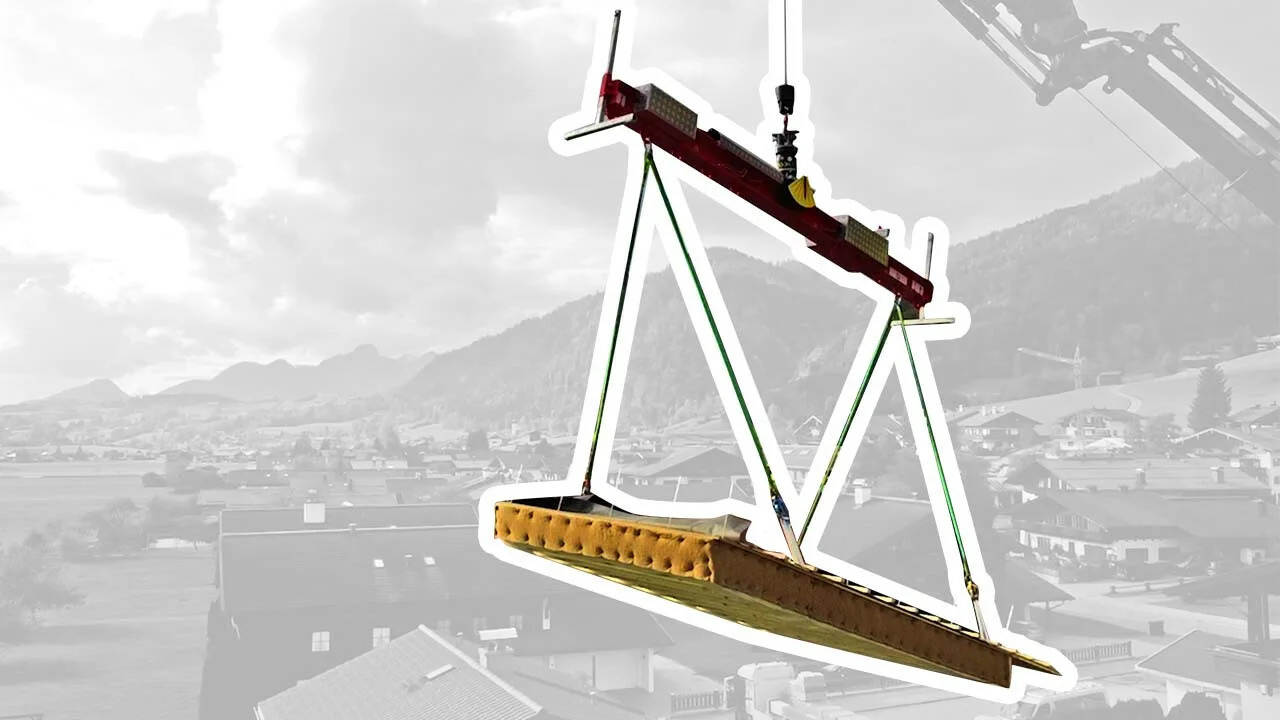
\includegraphics[width=0.5\textwidth]{graphics/Traverse.jpg}
    \caption{Ludwig Hook und Ludwig Traverse}
    \label{fig:ludwig}
\end{figure}

\subsubsection{Last}
Unter Lasten sind vor allem Fertigstrukturen wie z.B. Fertig erstellte Wände oder Dächer. 
Lasten haben maximal 2 Anschlagspunkte, welche einen Abstand von 1m bis 6m zueinander haben.
Diese Anschlagspunkte können auf unterschiedliche Höhen sein, wie z.B. bei Dächern welche eine
Neigung besitzen.

\subsubsection{Traverse}
Die LudwigTraverse ist eine Spezialtraverse, die speziell für den Lastausgleich entwickelt 
wurde. Sie erweist sich insbesondere dann als nützlich, wenn die Anschlagspunkte 
falsch positioniert sind und dadurch der Schwerpunkt der Last nicht korrekt berücksichtigt wird. 
Dies kann zu einer schrägen Ausrichtung beim Anheben der Last führen \cite{ludwigTraverse}.

\begin{figure}[H]
    \centering
    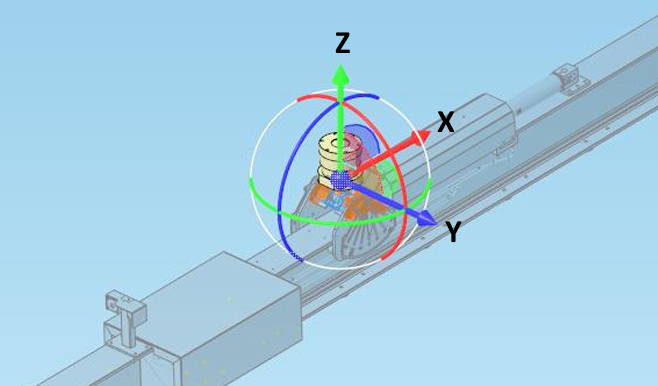
\includegraphics[width=0.5\linewidth]{graphics/Traverse_Rotationen.PNG}
    \caption{Koordinatensystem der Ludwig System Traverse}
    \label{fig:traverse}
\end{figure}

Abbildung \ref{fig:traverse} zeigt das linkshändige Koordinatensystem der Traverse.
Die Traverse hat Dimensionen (Länge × Breite × Höhe) von 500 cm × 70 cm × 50 cm.
Dabei wird fortan die Rotation um die Y-Achse der Traverse als Neigen definiert und die Rotation 
um die Z-Achse der Traverse als Rotieren definiert.

\subsection{Stand der Forschung}
Das Problem der Erkennung von Anschlagpunkten kann auf die Disziplin der Objektdetektion reduziert werden.
In der Arbeit von \cite{yong_object_2023} wird eine Methode vorgestellt, um mithilfe von Deep-Learning-Algorithmen 
in Kombination mit Ultraschallsensoren Unfälle auf Baustellen zu vermeiden. Diese Technologie wird genutzt, um die
Umgebung eines Krans zu überwachen und bei Bedarf einzugreifen. Das System integriert dabei eine Objekterkennung mit
einer Internet-Protokoll (IP)-Kamera zur Identifikation von Bauarbeitern im Gefahrenbereich und Ultraschallsensoren zur 
Messung von Abständen zu Hindernissen. Die Feldtests der entwickelten Lösung zeigten vielversprechende Ergebnisse, die 
zur Erhöhung der Sicherheit auf Baustellen beitragen können.


Eine weitere Arbeit, die den Nutzen von maschinellem Lernen auf Baustellen untersucht, ist \cite{zhou_image-based_2021}. 
In dieser Fallstudie wird ein KI-gestütztes, bildbasiertes Modell entwickelt, das Baustellenelemente erkennen und ihre 
Position bestimmen kann. Die vorgestellte Lösung kombiniert Ansätze wie Faster-R-CNN, Hough-Transformationen und eine Vertex-basierte
Bestimmungsmethode, um präzise Informationen zu Objekten, wie deren Koordinaten, Grösse und Farbe, zu extrahieren. Diese Daten werden
in einem BIM-Datenbankformat (Building Information Modeling) weiterverarbeitet, um die automatische Steuerung von Kränen zu unterstützen.
Der Ansatz stellt eine grundlegende Technologie für die Automatisierung von Kränen dar und fördert die Weiterentwicklung von Automatisierung 
und Robotik in der Bauindustrie.

\begin{figure}[H]
    \centering
    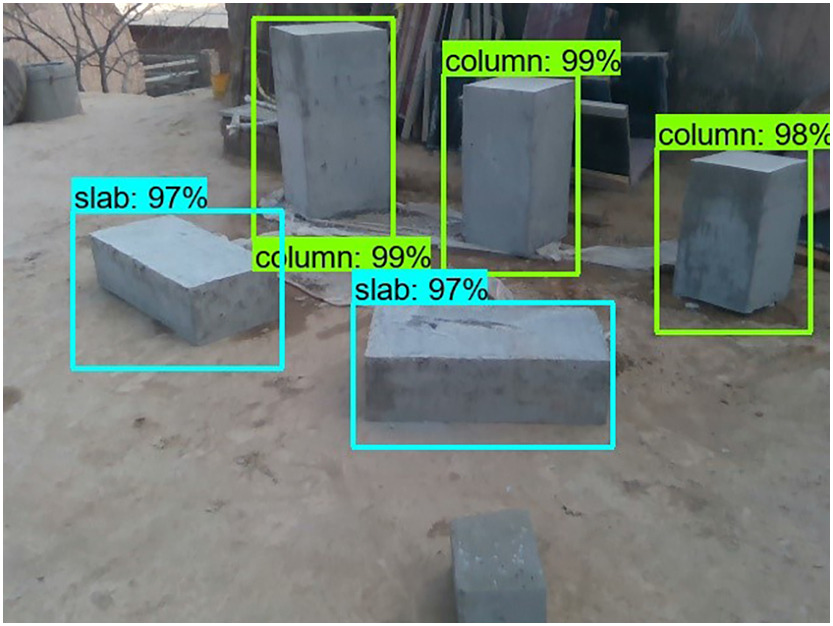
\includegraphics[width=0.6\linewidth]{object_reck.jpg}
    \caption{Ergebniss Foto des Objekterkennungsmodell von \cite{yong_object_2023}}
\end{figure}

Schliesslich untersucht die Arbeit von \cite{nasaMarkerReport} die Entwicklung und den Vergleich zweier Algorithmen zur Erkennung von 
Fiducial Markern. Ziel der Studie war es, mithilfe dieser Marker die Position und Orientierung des Roboters PUMA 560 präzise zu bestimmen. 
Die Marker bestehen aus einfachen geometrischen Formen wie Kreisen, Dreiecken und Quadraten. Die Arbeit vergleicht einen Algorithmus basierend 
auf Momentinvarianten mit einem zweiten, der eine diskrete Psi-S-Kurve verwendet. Letzterer erwies sich als überlegen und zeigte eine höhere 
Zuverlässigkeit bei der Marker-Erkennung. Diese Forschung liefert wertvolle Einblicke in die präzise Positionsbestimmung in Robotikanwendungen.

Um mit KI erfolgreich arbeiten zu können, ist ein Datensatz erforderlich, der bereits Bilder enthält, die korrekt markiert wurden. Solch ein Datensatz
wird genutzt, um ein KI-Modell zu trainieren. Leider konnten wir keinen Datensatz finden, der spezifisch auf unser Problem zugeschnitten ist. Ein eigener
Datensatz würde die Erstellung umfangreicher und zeitaufwendiger Annotationen erfordern, was den Rahmen dieses Projekts sprengen würde.

Zusätzlich müsste geprüft werden, ob die Kombination mit weiteren Sensoren wie Ultraschall- oder LiDAR-Kamerasystemen sinnvoll ist, um die Abstände sowie 
die Orientierung der Last und der Anschlagpunkte präzise zu bestimmen. Diese zusätzlichen Tests und Systeme wären jedoch mit Kosten verbunden und daher nicht praktikabel 
im Rahmen unserer aktuellen Ressourcen. Daher fokussieren wir uns darauf, die Position der Anschlagpunkte mithilfe von Fiducial Markern zu bestimmen.

\subsection{Fiducial Marker}
Fiducial Marker sind ein essenzielles Werkzeug in der modernen Bildverarbeitung und spielen eine 
zentrale Rolle in der räumlichen Orientierung und Positionsbestimmung. Insbesondere in Anwendungen 
wie der automatisierten Lastenhebung, wie sie von Ludwig System angestrebt wird, können Fiducial Marker 
helfen, Anschlagpunkte präzise zu lokalisieren.

Diese Marker, darunter Barcodes, QR-Codes oder speziell entwickelte AR-Marker, liefern visuelle 
Referenzen, die von Kamerasystemen erkannt und interpretiert werden können. Damit ermöglichen sie es, 
Objekte im Raum genau zu positionieren oder auszurichten.

In diesem Abschnitt untersuchen wir die Grundlagen von Fiducial Marker und beleuchten ihre spezifischen 
Einsatzmöglichkeiten in unserem Szenario, insbesondere im Kontext der automatisierten Ausrichtung von 
Anschlagpunkten auf der Traverse.

\subsubsection{Einführung Fiducial Marker}
Fiducial Marker sind quadratische Muster, die auf flachen Oberflächen aufgedruckt werden. 
Sie dienen als visuelle Referenzpunkte, die von Kamerasystemen erkannt und interpretiert 
werden können. Es gibt verschiedene Arten von Fiducial Marker, die je nach Anwendung 
unterschiedliche Eigenschaften und Einsatzmöglichkeiten bieten. 
Abbildung \ref{fig:marker_types} zeigt eine Auswahl solcher Marker.

\begin{figure}[H]
    \centering
    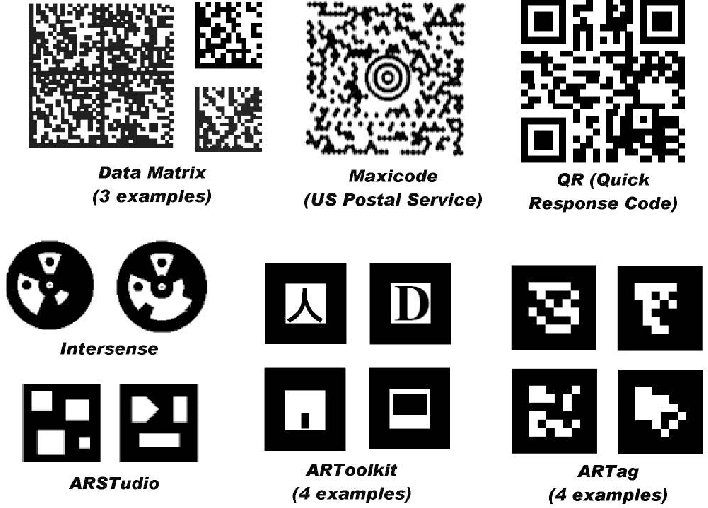
\includegraphics[width=0.7\linewidth]{graphics/marker_arten.png}
    \caption{Verschiedene Markerarten}
    \label{fig:marker_types}
\end{figure}

Grundsätzlich gilt: Je komplexer und grösser ein Marker ist, desto mehr Informationen können
darin gespeichert werden. Dabei muss jedoch der Informationsgehalt immer an die spezifischen 
Anforderungen der Anwendung angepasst werden, um eine optimale Balance zwischen Grösse, Lesbarkeit 
und Informationsdichte zu gewährleisten.

In der Robotik gehören AprilTags und AruCo-Marker zu den meistgenutzten Fiducial Marker. 
Ihre Beliebtheit basiert auf ihrer Robustheit und Effizienz bei der Lokalisierung in 
dreidimensionalen Räumen. Diese Marker wurden speziell entwickelt, um Verzerrungen und 
schwierige Lichtverhältnisse zu kompensieren und eine präzise Posenschätzung zu ermöglichen. 
Ihre Anwendung wird im weiteren Verlauf dieser Arbeit genauer beleuchtet, insbesondere im 
Kontext der automatisierten Lokalisierung von Anschlagpunkten.

\subsubsection {Wie AruCo und AprilTags erkannt werden}
AruCo-Marker und AprilTags sind quadratische Marker mit einem schwarzen Rand und einer binären Matrix, 
die spezifische Informationen wie die Marker ID encodiert. Der schwarze Rand erleichtert die schnelle Erkennung
der Marker in einem Bild, während die encodierte Matrix dazu dient, die ursprüngliche Orientierung
des Markers zu bestimmen. Die Grösse eines AruCo-Markers beeinflusst, wie viele Bits in der Matrix encodiert
werden können. Ein 4x4 AruCo-Marker besteht beispielsweise aus 16 Bits. Abbildung \ref{fig:sizes} zeigt 
Beispiele für verschiedene Grössen von AruCo-Markern. Der Marker unten rechts besteht aus einer 11x11-Matrix, 
was insgesamt 121 Bits ergibt.

\begin{figure}[H]
    \centering
    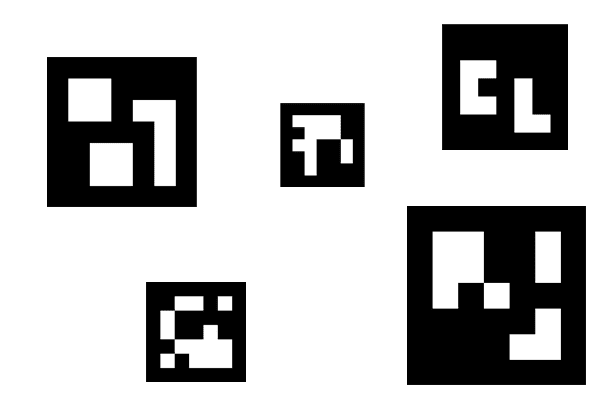
\includegraphics[width=0.6\linewidth]{marker_sizes.png}
    \caption{Unterschiedliche Grössen von AruCo-Markern im Vergleich}
    \label{fig:sizes}
\end{figure}


Um AruCo-Marker detektieren zu können, müssen zunächst Parameter wie die Anzahl der Quadrate, die die Matrix encodieren,
sowie die tatsächliche Grösse in der gewünschten Einheit angegeben werden. Der Erkennungsprozess erfolgt dabei in zwei 
Hauptschritten. Im ersten Schritt wird das Bild auf potenzielle Marker-Kandidaten analysiert. Dabei werden die Konturen
im Bild segmentiert und die Quadratischen Konturen bleiben für die weitere Verarbeitung erhalten. 
Konturen, die zu klein, zu gross oder zu nah beieinander liegen werden ebenfalls verworfen.
Abbildung \ref{fig:segmentation} zeigt eine Visualisierung des Segmentationsprozesses und wie potenzielle
Marker-Kandidaten identifiziert werden.

\begin{figure}[H]
    \centering
    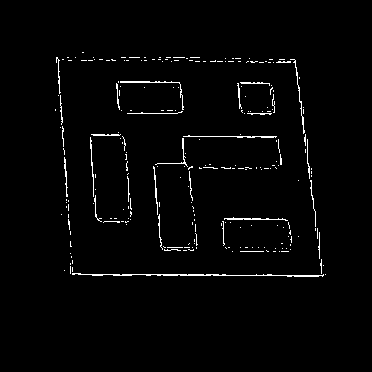
\includegraphics[width=0.6\linewidth]{segmentation.png}
    \caption{Kontur Segmentation eines Bildes}
    \label{fig:segmentation}
\end{figure}

Nachdem die Kandidaten ausgewählt wurden, muss in einem zweiten Schritt geprüft werden, ob es sich tatsächlich um Marker handelt.
Dazu werden aus dem kalibrierten Bild die einzelnen Bits eines Markers extrahiert. Um schwarze von weissen Bits unterscheiden zu können,
wird das Bild zuvor binarisiert. Der Schwellenwert für die Binarisierung wird mithilfe von Otsu's Methode bestimmt.

Im Anschluss wird das Bild in Zellen aufgeteilt, wobei die Zellgrösse durch die Markergrösse und die Anzahl der Bits eines Markers festgelegt
wird. Nachdem das Bild in Zellen unterteilt wurde, wird die Anzahl der schwarzen und weissen Pixel in jeder Zelle gezählt, um festzustellen, 
ob es sich bei der Zelle um ein schwarzes oder weisses Bit handelt.

Abschliessend wird überprüft, ob die extrahierten Bits mit dem vorgegebenen Dictionary übereinstimmen, sodass die Marker eindeutig zugeordnet werden können.

AprilTags folgen einem ähnlichen Ansatz, sind jedoch für höhere Genauigkeit und Robustheit optimiert. Ein zentraler Unterschied ist, dass AprilTags für eine
bessere Fehlerkorrektur ausgelegt sind, was sie besonders für Anwendungen in der Robotik und Augmented Reality geeignet macht.



\subsubsection{Posenschätzung durch AR Marker}
Das Problem der Posenberechnung stammt aus dem Bereich der erweiterten 
Realität. Dabei wird eine Gleichung gelöst, die den Projektionsfehler 
zwischen den 2D-Bildpunkten und den 2D-Projektionen der 3D-Weltpunkte minimiert. 
Das Lösen dieser Gleichung liefert einen Rotations- und Translationsvektor, der 
die Position und Orientierung der Kamera im Koordinatensystem beschreibt. 
Abbildung \ref{fig:pose} illustriert diesen Zusammenhang.

\begin{figure}[H]
    \centering
    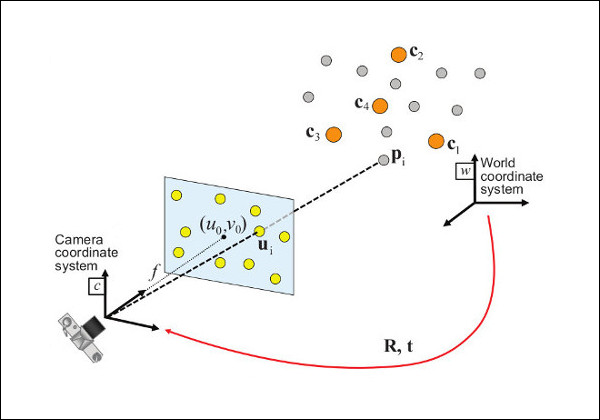
\includegraphics[width=0.4\linewidth]{graphics/pose.png}
    \caption{Posenschätzung}
    \label{fig:pose}
\end{figure}

Laut \cite{pose} braucht es dazu folgende Komponenten: die intrinsischen Parameter 
der Kamera \( K \) und die Projektionsmatrix \( \Pi \). Die intrinsischen Parameter 
können bereits vorher durch die Kalibrierung der Kamera berechnet werden. Die Kalibrierung 
wird mit OpenCV-Methoden durchgeführt, wie in \cite{zhang} und \cite{bradski} detailliert 
beschrieben.

Mithilfe der beiden Matrizen lässt sich eine Gleichung aufstellen, die \( N \) Punkte 
in der 3D-Welt auf 2D-Bildpunkte projiziert. Dabei entstehen die Rotationsmatrix und der 
Translationsvektor, die in der Transformationsmatrix \(\mathbf{T}^c_{w}\) enthalten sind.
Mit der Schätzung dieser Matrix können Weltkoordinaten in Kamerakoordinaten transformiert 
werden.

Gleichung um Weltkoordinaten im Bild zu projizieren:
\[
\begin{bmatrix}
u \\ 
v \\ 
1
\end{bmatrix}
=
\mathbf{A} \mathbf{\Pi} \mathbf{T}^c_{w}
\begin{bmatrix}
X_w \\ 
Y_w \\ 
Z_w \\ 
1
\end{bmatrix}
\]

\[
\begin{bmatrix}
u \\ 
v \\ 
1
\end{bmatrix}
=
\begin{bmatrix}
f_x & 0   & c_x & 0 \\ 
0   & f_y & c_y & 0 \\ 
0   & 0   & 1   & 0
\end{bmatrix}
\begin{bmatrix}
1 & 0 & 0 & 0 \\ 
0 & 1 & 0 & 0 \\ 
0 & 0 & 1 & 0
\end{bmatrix}
\begin{bmatrix}
r_{11} & r_{12} & r_{13} & t_x \\ 
r_{21} & r_{22} & r_{23} & t_y \\ 
r_{31} & r_{32} & r_{33} & t_z \\ 
0      & 0      & 0      & 1
\end{bmatrix}
\begin{bmatrix}
X_w \\ 
Y_w \\ 
Z_w \\ 
1
\end{bmatrix}
\]

Gleichung um Weltkoordinaten in Kamerakoordinaten zu transformieren:

\[
\begin{bmatrix}
X_c \\ 
Y_c \\ 
Z_c \\ 
1
\end{bmatrix}
=
\mathbf{T}^c_{w}
\begin{bmatrix}
X_w \\ 
Y_w \\ 
Z_w \\ 
1
\end{bmatrix}
\]

\[
\begin{bmatrix}
X_c \\ 
Y_c \\ 
Z_c \\ 
1
\end{bmatrix}
=
\begin{bmatrix}
r_{11} & r_{12} & r_{13} & t_x \\
r_{21} & r_{22} & r_{23} & t_y \\
r_{31} & r_{32} & r_{33} & t_z \\
0 & 0 & 0 & 1
\end{bmatrix}
\begin{bmatrix}
X_w \\ 
Y_w \\ 
Z_w \\ 
1
\end{bmatrix}
\]

\subsubsection{Probleme mit Fiducial Marker}
Mithilfe von Fiducial Marker können wir Anschlagpunkte erkennen und dessen Position bestimmen.
Zusätzlich können wir mit deren Hilfe ausrechnen wie sich die Traverse Positionieren musss, damit
sich über den den Anschlagspunkten befindent.

Allerdings stellen Fiducial Marker  keine perfekte Lösung dar, um Anschlagpunkte zuverlässig zu lokalisieren. 
Sie sind besonders empfindlich gegenüber äusseren Einflüssen. Bereits geringe Verschmutzungen, 
wie etwa Schmutz oder Staub auf den Kanten, können die Erkennung erheblich beeinträchtigen 
oder sogar vollständig verhindern.

Darüber hinaus sind Fiducial Marker anfällig für ungünstige Lichtverhältnisse. Blendung, Schatten 
oder Reflexionen können die Erkennungsrate deutlich verringern, insbesondere in Aussenbereichen 
oder bei wechselnden Lichtbedingungen. Auch der Erkennungsbereich der Marker ist begrenzt: Marker 
müssen sich in einem bestimmten Abstand und Winkel zur Kamera befinden um erkannt zu werden.

Grössere Marker können zwar leichter erkannt werden, bringen jedoch eigene Herausforderungen mit sich. 
insbesondere wenn auf der Last nicht genügend Platz für die Anbringung verfügbar ist. Zudem nutzen 
sich Marker durch äussere Einflüsse, wie Witterung oder mechanische Belastung, schnell ab. Um die 
Erkennung dauerhaft zu gewährleisten, müssen sie regelmässig ersetzt oder neu angebracht werden.


\clearpage
\subsection{Kameras}
Um die Anschlagpunkte zuverlässig erkennen zu können, sind geeignete Kamerasysteme
erforderlich. Um zu verstehen, warum bestimmte Schritte, wie beispielsweise die 
Kalibrierung der Kamera, notwendig sind und warum es zu Ungenauigkeiten bei den 
Berechnungen zur Positionierung der Traverse kommen kann, betrachten wir in diesem 
Abschnitt die Funktionsweise und Eigenschaften von Kamerasystemen genauer.

\subsubsection{Kameraeigenschaften}
Eine Kamera kann ein Bild generieren, das insgesamt \( L \) Pixel in 
der Länge und \( H \) Pixel in der Höhe besitzt. \( L \) und \( H \) 
beschreiben hierbei die Auflösung der Kamera. Die Auflösung ist ein 
wichtiger Faktor, da sie bestimmt, wie viele Details in einem Bild 
sichtbar sind. Höhere Auflösungen ermöglichen genauere Berechnungen, 
erfordern jedoch auch mehr Rechenleistung für die Verarbeitung der 
Bilder.

Das FOV (Field of View) einer Kamera beschreibt den Bereich der Szene,
den die Kamera sehen oder aufnehmen kann. Es ist ein grundlegender 
Parameter, der angibt, wie viel von der Umgebung eine Kamera in einem 
Bild oder Video erfassen kann. Je höher das FOV, desto grösser ist 
jedoch die Verzerrung, die im Bild entsteht.
Abbildung \ref{fig:fisheye} zeigt, wie eine starke Verzerrung aussieht,
die typischerweise bei Weitwinkel- oder Fisheye-Objektiven auftritt.

\begin{figure}[H]
    \centering
    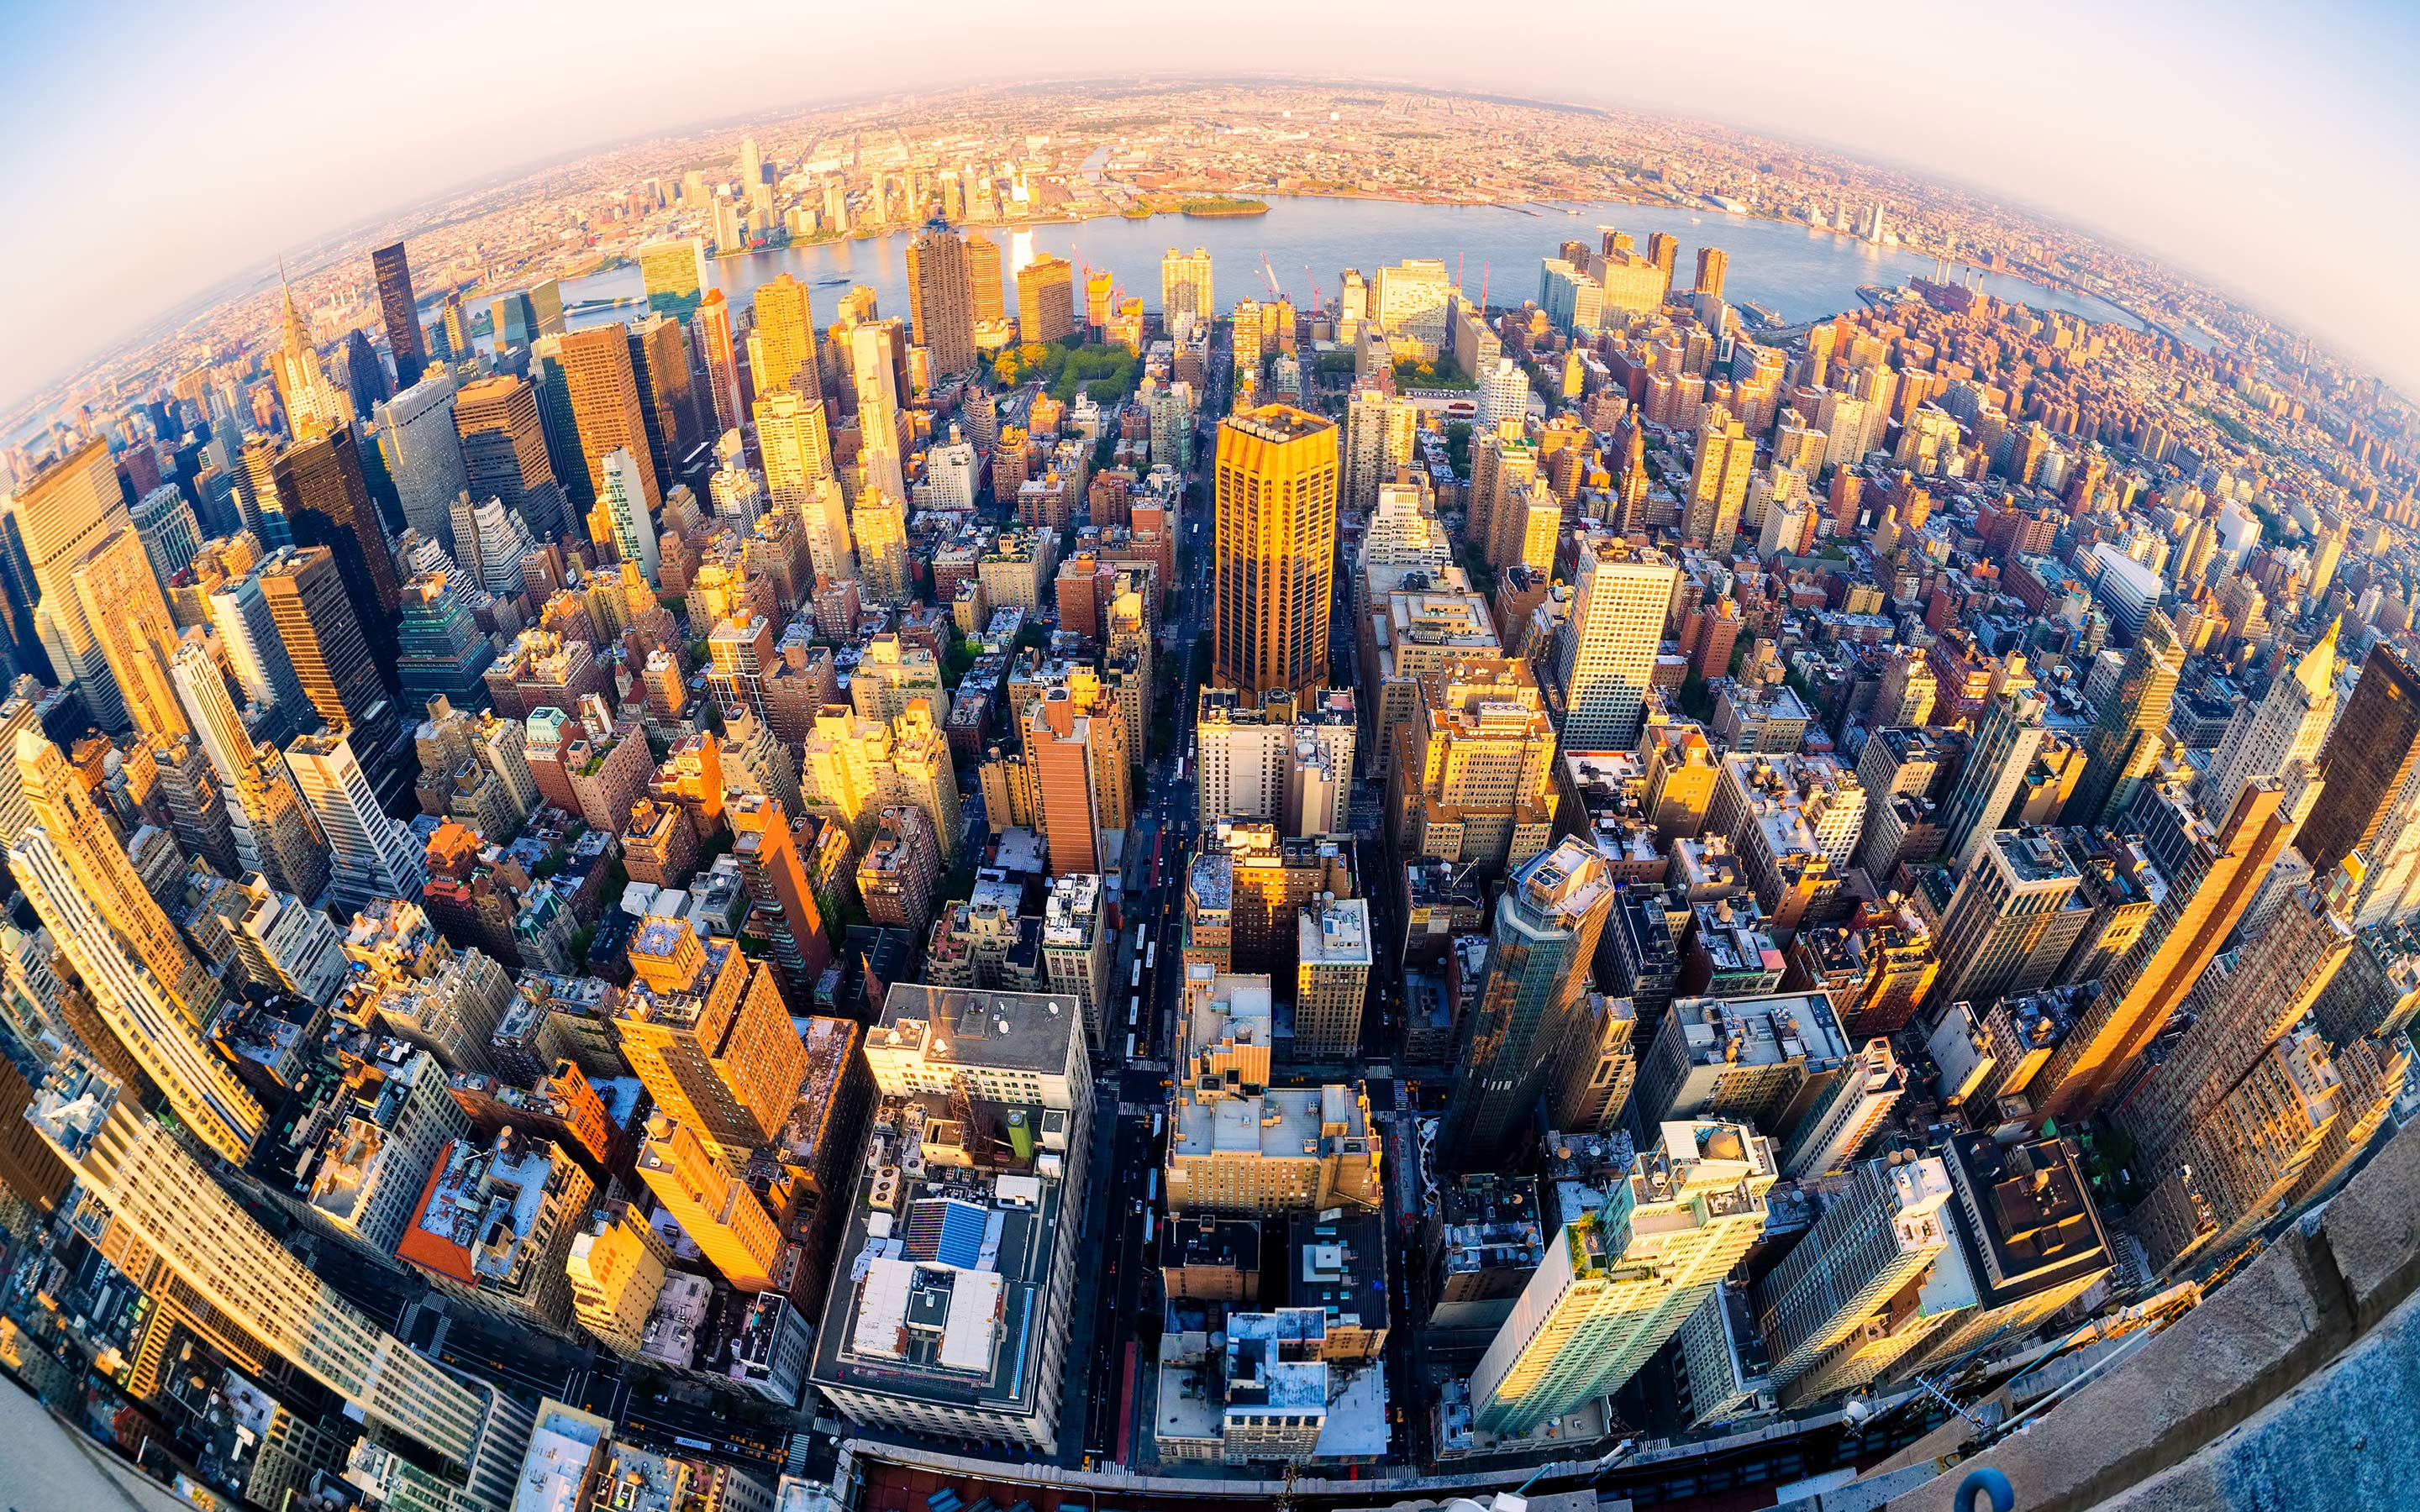
\includegraphics[width=0.5\linewidth]{graphics/fisheye.jpg}
    \caption{Beispielfoto einer starken Verzerrung}
    \label{fig:fisheye}
\end{figure}

Neben Auflösung und FOV gibt es weitere wichtige Eigenschaften, die 
bei der Auswahl und Nutzung einer Kamera berücksichtigt werden sollten:

\begin{itemize}
    \item \textbf{Bildrate (Frame Rate):} Gibt an, wie viele Bilder pro Sekunde aufgenommen werden können.
    \item \textbf{Fokus und Tiefenschärfe:} Der Fokusbereich beeinflusst, welche Bereiche des Bildes scharf dargestellt werden.
\end{itemize}


\subsubsection{Intrinsische Kalibrierung}
Verzerrungen, insbesondere an den Kanten eines Bildes, können zu Rechenfehlern 
bei der Positionierung der Traverse führen. Verzerrungen entstehen durch optische 
Abweichungen der Linse und sind besonders bei hohen FOV-Werten ausgeprägt. 
Zudem können sie die Erkennung der Anschlagpunkte erschweren, da die Form und 
Lage der Marker falsch interpretiert werden können.

Es gibt zwei Hauptarten von Verzerrungen bei Kameralinsen: die radiale und die tangentiale Verzerrung.
Die radiale Verzerrung führt dazu, dass eigentlich gerade Linien gekrümmt erscheinen. Abbildung 
\ref{fig:distortion} verdeutlicht die Auswirkung der radiale Verzerrung, bei der gerade Linien gekrümmt
dargestellt werden.

\begin{figure}[H]
    \centering
    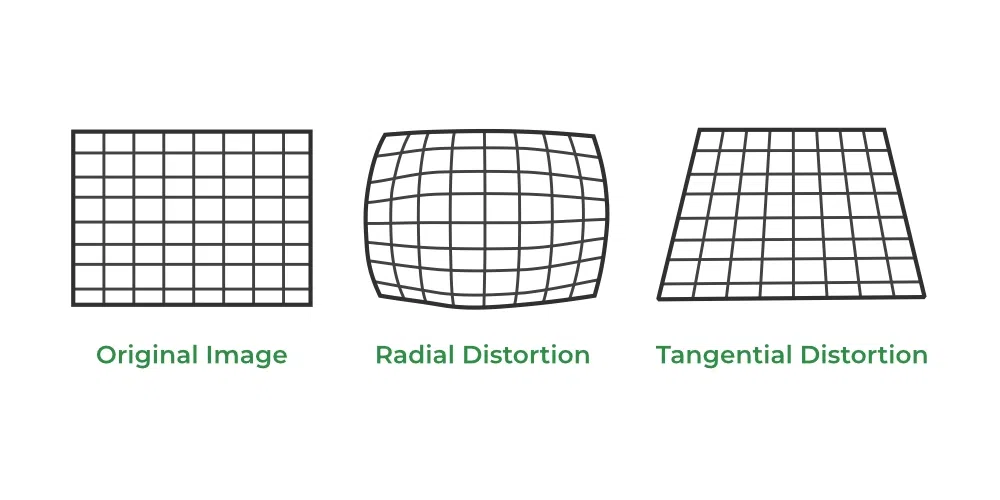
\includegraphics[width=\linewidth]{distortion.png}
    \caption{Beispiele von Verzerrungen}
    \label{fig:distortion}
\end{figure}

Die tangentiale Verzerrung entsteht, wenn die Kameralinse nicht perfekt parallel zur Bildebene ausgerichtet
ist. Dies führt dazu, dass bestimmte Bereiche des Bildes näher erscheinen als andere, wodurch eine ungleichmässige
Darstellung entsteht. 

Die radiale Verzerrung lässt sich mit folgender Formel berechnen:

\[
x_\text{distorted} = x(1 + k_1r^2 + k_2r^4 + k_3r^6) \quad
y_\text{distorted} = y(1 + k_1r^2 + k_2r^4 + k_3r^6)
\]

Die Formel zur Berechnung der tangentialen Verzerrung lautet:

\[
x_\text{distorted} = x + \left[ 2p_1xy + p_2(r^2 + 2x^2) \right]
y_\text{distorted} = y + \left[ p_1(r^2 + 2y^2) + 2p_2xy \right]
\]

Das \(r\) ist hierbei für den euklidischen der Abstand den ein Pixel mit Koordinaten \((x, y)\) zum Bildzentrum hat.
Zusammengefasst muss man also die Verzerrungskoeffizienten k1, k2, p1, p2 und k3 finden.

\[
Verzerrungskoeffizienten = (k1, k2, p1, p2, k3)
\]

Zusätzlich zu den Verzerrungskoeffizienten werden auch die intrinsischen Parameter der Kamera benötigt. Diese können 
mithilfe eines vorgegebenen Kalibrierungsmusters berechnet werden. Dabei werden bekannte Punkte des Musters verwendet,
deren tatsächliche Positionen in Weltkoordinaten bekannt sind. Anschliessend werden diese Punkte auf die Bildkoordinaten
projiziert. Die Kalibrierung minimiert iterativ den Reprojektion-Fehler, der die Differenz zwischen den projizierten 
Punkten und den gemessenen Bildpunkten darstellt.

\[
K =
\begin{bmatrix}
f_x & 0 & c_x \\
0 & f_y & c_y \\
0 & 0 & 1
\end{bmatrix}
\]

Die Kamerakalibrierung umfasst die Korrektur von Verzerrungen sowie die Bestimmung der 
intrinsischen Parameter der Kamera, wie:

\begin{itemize}
    \item \textbf{Brennweite} (\( f_x, f_y \)): Gibt an, wie stark die Linse das Licht bündelt.
    \item \textbf{Hauptpunkt} (\( c_x, c_y \)): Die Koordinaten des optischen Zentrums auf dem Bildsensor.
    \item \textbf{Verzerrungskoeffizienten}: Parameter, die die Stärke der Verzerrungen beschreiben.
\end{itemize}


Um eine Kamera zu kalibrieren, werden mehrere Fotos eines regelmässigen Musters 
benötigt. Die Bilder sollten aus verschiedenen Distanzen und Blickwinkeln aufgenommen werden,
um eine möglichst breite Datenbasis zu schaffen. Dabei ist es wichtig die Kamera zu bewegen, während
das Muster fest positioniert bleibt. Abbildung \ref{fig:corrected} zeigt die Korrektur von Verzerrungen
anhand eines Kalibrierungsmusters, wobei die Verzerrung vor und nach der Kalibrierung sichtbar ist.

\begin{figure}[H]
    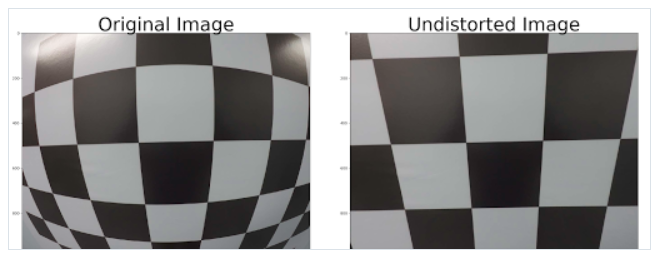
\includegraphics[width=\linewidth]{corrected.png}
    \caption{Muster vor und nach der Kalibrierung}
    \label{fig:corrected}
\end{figure}

Die Dokumentation von OpenCV \cite{opencv_calibration_tutorial} liefert praktische 
Beispiele und erklärt detailliert, wie die Kalibrierung implementiert werden 
kann.


\subsection{Benutzte Frameworks}
OpenCV ist eine populäre Open-Source-Bibliothek für verschiedene Bildverarbeitungssoftware.
Open Source bedeutet, dass die Funktionen für jeden frei verfügbar sind. OpenCV bietet 
umfangreiche Funktionen, um AruCo-Marker zu erkennen und eine Kamerakalibration durchzuführen.
Weitere Informationen zu OpenCV finden sich auf der offiziellen Webseite unter opencv.org.

Allerdings unterstützt OpenCV keine Erkennung von AprilTags. Um diese Aufgabe zu erfüllen, verwenden 
wir stattdessen eine spezielle Ressource, die im GitHub-Repository für AprilTags bereitgestellt 
wird \cite{apriltag_github}. Dieses Repository basiert auf drei wissenschaftlichen Arbeiten 
\cite{olson2011tags} \cite{wang2016iros} \cite{krogius2019iros} und bietet eine effiziente 
und robuste Lösung zur Erkennung von AprilTags. Die Software wird unter der BSD 2-Clause License 
veröffentlicht, die eine freie Nutzung, Modifikation und Weiterverteilung unter bestimmten Bedingungen 
erlaubt. Weitere Details zur Lizenz können direkt im Repository nachgelesen werden.